\documentclass[12pt,a4paper]{article}

\usepackage[utf8]{inputenc}
\usepackage[brazilian]{babel}
\usepackage{amsmath}
\usepackage{graphicx}
\usepackage{siunitx}
\usepackage{booktabs}
\usepackage{geometry}
\usepackage{float}

\usepackage[authoryear]{natbib}

\geometry{margin=2.5cm}

\title{Determinação da Aceleração da Gravidade por Meio do Experimento de Queda Livre}
\author{Enzo Rocha Leite Diniz Ribas \\ Centro Federal de Educação Tecnológica de Minas Gerais}
\date{\today}

\begin{document}
\begin{titlepage}

\begin{center}


\includegraphics[width=4cm]{media/Logo_CEFET-MG.png}

\Large
Centro Federal de Educação Tecnológica de Minas Gerais

\vspace{1cm}

\Large
Curso de Engenharia Mecânica

\vspace{2cm}

\Huge
Determinação da Aceleração da Gravidade por Meio do Experimento de Queda Livre

\vspace{3cm}

\begin{flushright}
\Large
Mecânica, Oscilações, Fluidos e Termodinâmica, Turma 6T56 \\
Prof. Dr. Mauro Lucio Lobão Iannini
\end{flushright}

\vspace{3cm}

\large
Enzo Rocha Leite Diniz Ribas (Eng. Mecânica - 20253002819)\\
Gabriel Resende Amorim Oliveira (Eng. Elétrica - 20233014438)\\
Leandro Césari e Silva Barros (Eng. Mecânica - 20253005104)\\

\vfill

\Large
Belo Horizonte

\Large
\the\year/{1}

\end{center}

\end{titlepage}

\section{Introdução}

O experimento de queda livre constitui um dos métodos clássicos para a determinação da aceleração da gravidade. A análise do movimento de um corpo submetido exclusivamente à ação da gravidade permite verificar experimentalmente as relações previstas pela cinemática do movimento uniformemente acelerado.

Neste experimento tem-se como objetivo determinar o valor local, em módulo, da aceleração da gravidade a partir da análise do tempo de queda de uma esfera metálica liberada a partir de diferentes alturas. Os dados experimentais foram analisados por meio de diferentes métodos de ajuste e linearização, permitindo comparar os resultados obtidos.

\section{Fundamentação Teórica}

Quando um objeto é abandonado a partir do repouso e submetido apenas à força gravitacional, ele realiza um movimento retilíneo uniformemente acelerado, no qual a aceleração é a mesma para todos os corpos, desprezando pequenas variações decorridas de fatores como a altitude e a latitude \citep{moyses2013}. A equação do movimento é dada por 
\begin{equation}
h(t) = h_0 + v_0 t + \frac{1}{2} g t^2
\label{eq:movimento}
\end{equation}
em que $h_0$ é a altura inicial, $h(t)$ é a altura do objeto no instante $t$, $t$ é o tempo de queda, $v_0$ é a velocidade inicial, $g$ é a aceleração da gravidade.

\section{Metodologia}

O experimento foi realizado utilizando um sistema composto por um sensor óptico e um eletroímã conectados a um cronômetro eletrônico, Figuras ~\ref{fig:setup} e ~\ref{fig:measuring_device}. Uma esfera metálica foi liberada a partir de diferentes alturas e o tempo de queda foi registrado.

\begin{figure}[H]
\centering
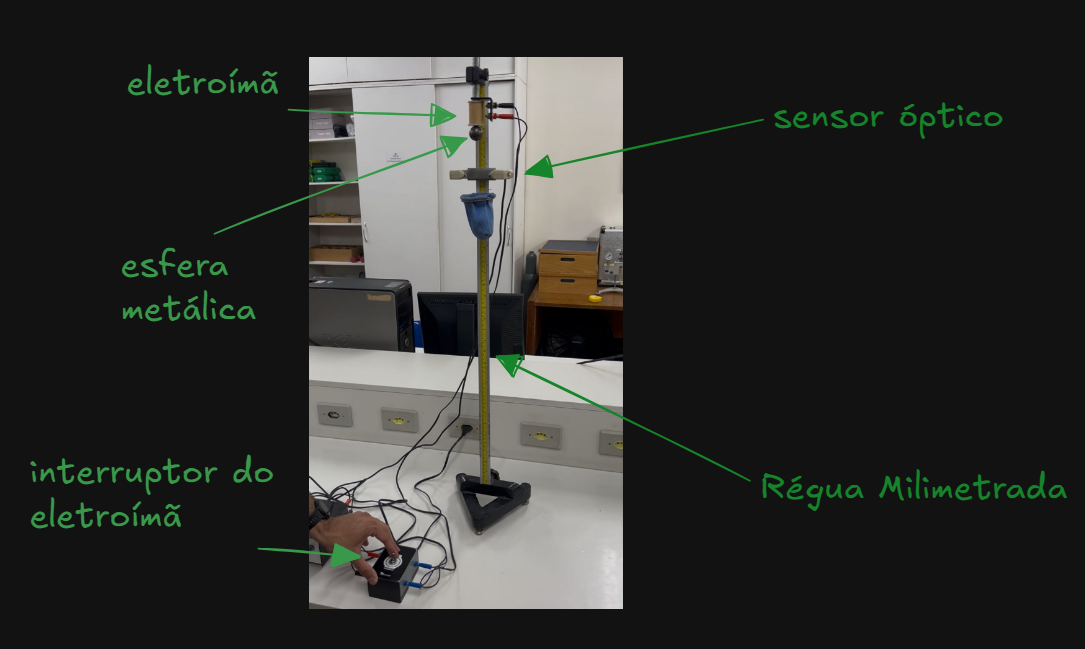
\includegraphics[width=0.7\textwidth]{media/photos/sensor_with_ruller_setas.png}
\caption{Sistema experimental utilizado para a determinação da aceleração da gravidade.}
\label{fig:setup}
\end{figure}

\begin{figure}[H]
\centering
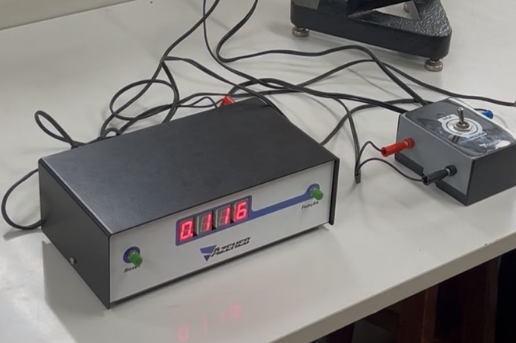
\includegraphics[width=0.7\textwidth]{media/photos/measuring_device.png}
\caption{Cronométro eletrônico utilizado para registrar o tempo de queda da esfera.}
\label{fig:measuring_device}
\end{figure}

O sensor óptico foi posicionado de forma a detectar a passagem da esfera, permitindo o registro preciso do tempo de queda. O eletroímã foi utilizado para manter a esfera suspensa até o momento da liberação, garantindo que a velocidade inicial fosse nula. O sistema calcula automaticamente o tempo decorrido entre a liberação da esfera e a detecção pelo sensor, exibindo o resultado em um display digital com até três casas decimais de precisão.

Foram selecionadas diferentes alturas ao longo da régua disponível, cobrindo uma faixa ampla de valores. Para cada altura, registrou-se o tempo correspondente à passagem da esfera entre os sensores.

Os dados foram organizados em tabela e analisados utilizando o software SciDAVis para geração de gráficos e realização de ajustes de curvas.

\section{Procedimentos}

O procedimento experimental seguiu as seguintes etapas:

\subsubsection{Ajuste de posições dos sensores e do eletroímã}
A esfera metálica foi posicionada em um ponto fixo. O sensor óptico teve sua posição ajustada em diferentes alturas para detectar a passagem da esfera.

\subsubsection{Liberação da esfera a partir do repouso}
A esfera foi liberada a partir do repouso, garantindo que a velocidade inicial fosse nula.

\subsubsection{Registro do tempo de queda utilizando sensores ópticos}
O tempo de queda foi registrado automaticamente pelo sistema de sensores ópticos, que detecta a passagem da esfera e exibe o resultado em um display digital.

\subsubsection{Repetição das medições para diferentes alturas}
Foram feitas 3 medições para cada uma das 9 alturas selecionadas, totalizando 27 medições. As alturas escolhidas foram: 0.05 m, 0.08 m, 0.12 m, 0.15 m, 0.18 m, 0.2 m, 0.3 m, 0.36 m e 0.64 m, em relação à posição inicial.

\subsubsection{Organização dos dados em tabela}
Foi feita uma média aritmética dostempos registrados para cada altura, e os valores médios foram utilizados para a análise dos dados.

\subsubsection{Construção de gráficos e realização de ajustes no SciDAVis}
Os dados organizados em tabela foram importados para o software SciDAVis para análise de dados. No experimento, a esfera é abandonada a partir do repouso e  o ponto de liberação como origem das posições, a equação \eqref{eq:movimento} do movimento torna-se
\begin{equation}
h_0 = 0; v_0 = 0 \implies h = \frac{1}{2} g t^2
\end{equation}
A partir dessa equação podem ser construídas diferentes representações gráficas para determinação experimental de $g$.

A primeira possibilidade consiste em analisar o gráfico da altura em função do tempo, $h$ vs $t$, o que resulta em um comportamento parabólico do tipo
\begin{equation*}
h(t) = A t^2
\end{equation*}
no qual o coeficiente $A$ corresponde a $g/2$, logo $g = 2A$. Na forma original, a equação é dada por
\begin{equation}
h(t) = \frac{g}{2} t^2.
\label{eq:quadratic}
\end{equation}

Pelo ajuste não linear dos dados no gráfico $h$ vs $t$, o valor de $g$ pode ser determinado a partir do coeficiente do termo quadrático. Mas essa representação não é a mais adequada para a determinação de $g$ a partir de um ajuste de curva, pois envolve o ajustes não lineares que necessitam métodos iterativos e uma boa estimativa inicial, enquanto ajustes lineares podem ser resolvidos de forma mais simples e direta \citep{bevington2003data}.

Portanto, uma forma de linearização do movimento é definir \(z = t^2\), de modo que o gráfico da altura \(h\) em função de \(z\) resulte em uma relação linear:

\begin{equation*}
h(z) = A z + b,
\end{equation*}

onde \(A = \frac{g}{2}\) é o coeficiente angular da reta e \(b\) é um deslocamento fixo que corrige a posição inicial medida pelo sensor, já que o ponto exato de detecção não pode ser definido com precisão. Em termos de \(t\), a relação original é

\begin{equation}
h(t) = \frac{g}{2} t^2 + b.
\label{eq:linearized_with_t2}
\end{equation}

A partir do ajuste linear dos dados no gráfico \(h\) vs \(t^2\), o valor da aceleração da gravidade pode ser determinado a partir do coeficiente angular, usando

\begin{equation*}
A = \frac{g}{2} \implies g = 2A.
\end{equation*}

Outra possibilidade de linearização consiste em definir \(w = \sqrt{h}\), de modo que o gráfico do tempo \(t\) em função de \(w\) também resulte em uma relação linear:

\begin{equation*}
t(w) = A w + b,
\end{equation*}

onde \(A = \sqrt{\frac{2}{g}}\) é o coeficiente angular e \(b\) representa novamente o deslocamento fixo do sensor. Em termos de \(h\), a relação original é

\begin{equation}
t(h) = \sqrt{\frac{2}{g}} \sqrt{h} + b.
\label{eq:linearized_with_sqrt_h}
\end{equation}

Pelo ajuste linear dos dados no gráfico \(t\) vs \(\sqrt{h}\), a aceleração da gravidade pode ser obtida a partir de

\begin{equation*}
A = \sqrt{\frac{2}{g}} \implies g = \frac{2}{A^2}.
\end{equation*}


\section{Discussão e Análise dos Resultados}

A Tabela ~\ref{tab:experimental_data} apresenta os valores experimentais obtidos.

\begin{table}[h]
\centering
\begin{tabular}{cc}
\toprule
\textbf{Tempo Médio $t$ (s)} & \textbf{Altura $h$ (m)} \\
\midrule
0,115 & 0,05 \\
0,141 & 0,08 \\
0,168 & 0,12 \\
0,186 & 0,15 \\
0,203 & 0,18 \\
0,212 & 0,20 \\
0,257 & 0,30 \\
0,280 & 0,36 \\
0,370 & 0,64 \\
\bottomrule
\end{tabular}
\caption{Dados experimentais de altura e tempo de queda.}
\label{tab:experimental_data}
\end{table}

\subsection{Gráfico $h$ versus $t$}

O gráfico da altura em função do tempo, ilustrado na Figura ~\ref{graph1_quadratic_fit}, apresenta comportamento parabólico, conforme esperado teoricamente.

\begin{figure}[H]
\centering

\includegraphics[width=0.7\textwidth]{media/graph1_quadratic_fit.pdf}
\caption{Altura em função do tempo de queda.}
\label{graph1_quadratic_fit}
\end{figure}

O ajuste da curva utilizando a equação quadrática \eqref{eq:quadratic} forneceu um valor para a aceleração da gravidade de
\begin{equation}
g_1 = 9,56 \pm 0,020 \;\text{m/s}^2
\end{equation}

\subsubsection{Log do SciDAVis}
\begin{verbatim}
[sábado, 21 de março de 2026 00:57:15 Hora oficial do Brasil	Plot: ''Graph1'']
Non-linear fit of dataset: Table1_h, using function: a/2*x^2+b
Y standard errors: Unknown
Scaled Levenberg-Marquardt algorithm with tolerance = 0,0001
From x = 0,115 to x = 0,37
a  = 9,56088505838644 +/- 0,0200645333473526
b  = -0,0150434356031264 +/- 0,000630362266036001
--------------------------------------------------------------------------------------
Chi^2 = 8,22150810757668e-06
R^2 = 0,999988999855355
---------------------------------------------------------------------------------------
Iterations = 1
Status = success
---------------------------------------------------------------------------------------
\end{verbatim}

\subsection{Linearização $h$ versus $t^2$}

A linearização dos dados permitiu obter uma relação aproximadamente linear, ilustrada no gráfico da Figura ~\ref{graph2_linearization_hoft2}.

\begin{figure}[H]
\centering
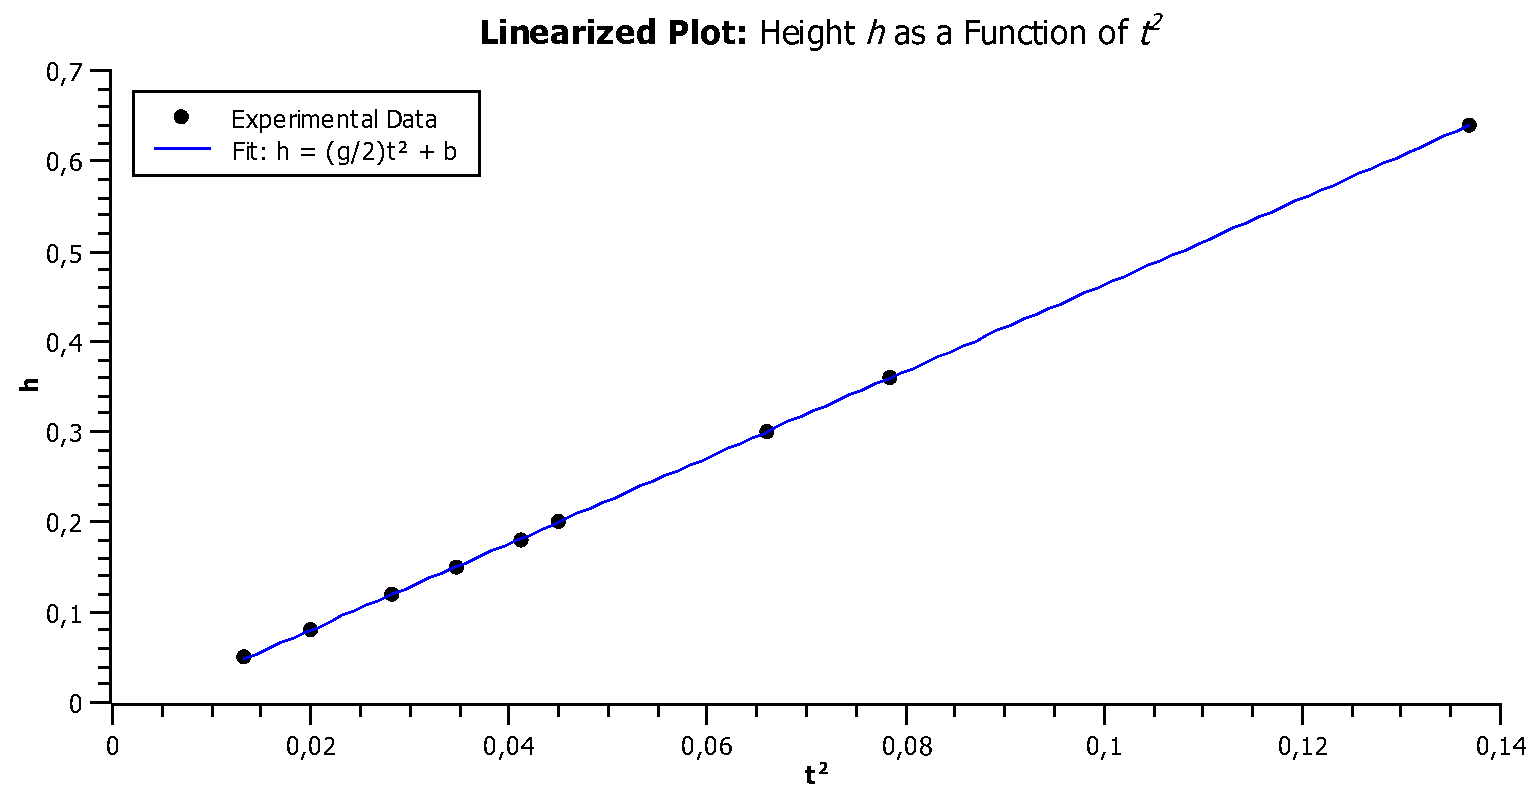
\includegraphics[width=0.7\textwidth]{media/graph2_linearization_hoft2.pdf}
\caption{Gráfico linearizado $h$ em função de $t^2$.}
\label{graph2_linearization_hoft2}
\end{figure}

O ajuste linear a partir da equação de linearização ~\eqref{eq:linearized_with_t2} forceneu um valor para a aceleração da gravidade de
\begin{equation}
g_2 = 9,56 \pm 0,02 \; \text{m/s}^2
\end{equation}

\subsubsection{Log do SciDAVis}
\begin{verbatim}
[sábado, 21 de março de 2026 00:57:48 Hora oficial do Brasil	Plot: ''Graph2'']
Non-linear fit of dataset: Table1_h, using function: a/2*x+b
Y standard errors: Unknown
Scaled Levenberg-Marquardt algorithm with tolerance = 0,0001
From x = 0,013225 to x = 0,1369
a  = 9,56088505838644 +/- 0,0200645333473526
b  = -0,0150434356031264 +/- 0,000630362266036001
--------------------------------------------------------------------------------------
Chi^2 = 8,22150810757668e-06
R^2 = 0,999988999855355
---------------------------------------------------------------------------------------
Iterations = 1
Status = success
---------------------------------------------------------------------------------------
\end{verbatim}

\subsection{Linearização $t$ versus $\sqrt{h}$}

A linearização dos dados utilizando a raiz quadrada da altura também resultou em uma relação aproximadamente linear, ilustrada no gráfico da Figura ~\ref{graph3_linearization_tofsqrt_h},

\begin{figure}[H]
\centering
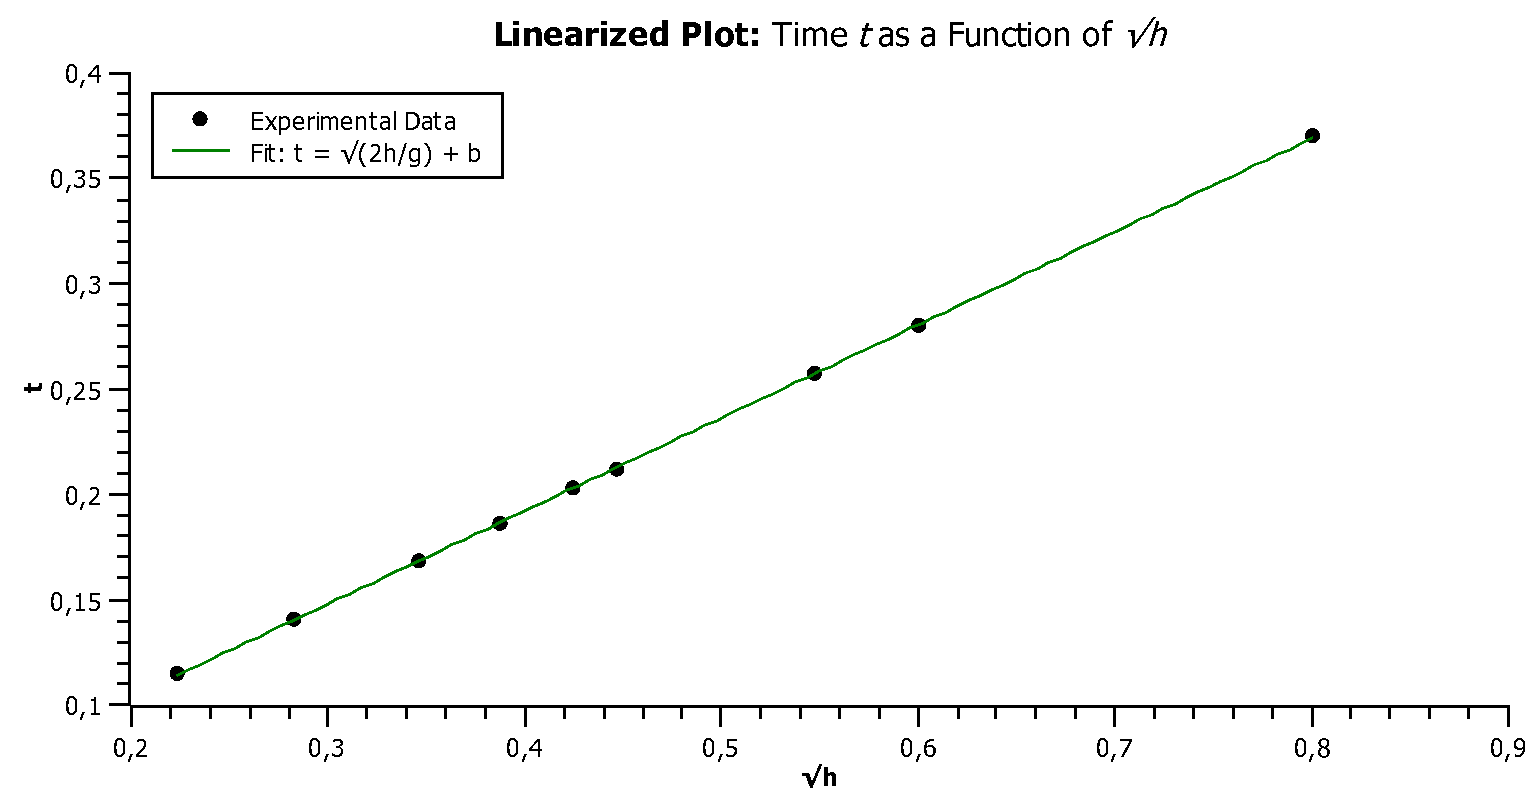
\includegraphics[width=0.7\textwidth]{media/graph3_linearization_tsqrth.pdf}
\caption{Tempo em função da raiz quadrada da altura de queda.}
\label{graph3_linearization_tofsqrt_h}
\end{figure}

que a partir do ajuste linear da equação ~\eqref{eq:linearized_with_sqrt_h} forneceu um valor para a aceleração da gravidade de
\begin{equation}
g_3 = 10,23 \pm 0,07 \; \text{m/s}^2
\end{equation}

\subsubsection{Log do SciDAVis}

\begin{verbatim}
[sábado, 21 de março de 2026 00:58:58 Hora oficial do Brasil	Plot: ''Graph3'']
Non-linear fit of dataset: Table1_t, using function: sqrt(2/a)*x + b
Y standard errors: Unknown
Scaled Levenberg-Marquardt algorithm with tolerance = 0,0001
From x = 0,223606797749979 to x = 0,8
a  = 10,2312232033732 +/- 0,07185180503817
b  = 0,0152478719128495 +/- 0,000746348656072025
--------------------------------------------------------------------------------------
Chi^2 = 4,2022153033684e-06
R^2 = 0,999990932323245
---------------------------------------------------------------------------------------
Iterations = 6
Status = success
---------------------------------------------------------------------------------------
\end{verbatim}

\section{Propagação de Incertezas}
A estimativa da incerteza para uma grandeza derivada $f(x_1, x_2, \dots, x_n)$ é fundamentada na expansão em série de Taylor de primeira ordem, assumindo que as fontes de erro são independentes e aleatórias. A incerteza combinada é dada por
\begin{equation}
    \Delta f = \sqrt{
        \sum_{i=1}^{n} 
        \left( \frac{\partial f}{\partial x_i} \Delta x_i \right)^2
        }
\end{equation}

\subsection{Análise por Ponto Experimental (Cálculo Indireto)}
Para o cálculo de $g$ em cada ponto individual utilizando a relação $g = 2h/t^2$, a propagação das incertezas instrumentais ($\Delta h = \SI{0,005}{\meter}$ e $\Delta t = \SI{0,0005}{\second}$) resulta na incerteza relativa
\begin{equation}
    \frac{\Delta g}{g} = 
    \sqrt{
        \left(\frac{\Delta h}{h}\right)^2 + 
        \left(2 \frac{\Delta t}{t}\right)^2
        }
        \label{eq:incerteza_relativa}
\end{equation}
Esta expressão revela que o erro no tempo é quadraticamente mais impactante que o erro na altura. Apesar disso, para alturas pequenas, a incerteza relativa é dominada pelo erro na altura, enquanto para alturas maiores, o erro no tempo torna-se mais significativo. Para a menor altura medida o erro relativo é
\begin{equation*}
    \frac{\Delta g}{g} = \sqrt{
        \left(\frac{0{,}005}{0{,}05}\right)^2 + 
        \left(2 \frac{0{,}0005}{0{,}115}\right)^2
        } \approx 0{,}1
\end{equation*}
enquanto para a maior altura o erro relativo é
\begin{equation*}
    \frac{\Delta g}{g} = \sqrt{
        \left(\frac{0{,}005}{0{,}64}\right)^2 + 
        \left(2 \frac{0{,}0005}{0{,}370}\right)^2
        } \approx 0{,}01
\end{equation*}
indicando que a incerteza relativa diminui significativamente com o aumento da altura.

\begin{table}[H]
\centering
\caption{Cálculo da aceleração da gravidade local e incertezas associadas para cada ponto experimental.}
\label{tab:calculo_ponto_a_ponto}
\begin{tabular}{c c S[table-format=1.2, table-figures-uncertainty=1]}
\toprule
\textbf{Altura $h$ (m)} & \textbf{Tempo $t$ (s)} & {\textbf{Aceleração $g \pm \Delta g$ (m/s$^2$)}} \\
\midrule
0,05 & 0,115 & 9.45 \pm 0.95 \\
0,08 & 0,141 & 8.05 \pm 0.55 \\
0,12 & 0,168 & 8.50 \pm 0.40 \\
0,15 & 0,186 & 8.66 \pm 0.30 \\
0,18 & 0,203 & 8.73 \pm 0.25 \\
0,20 & 0,212 & 8.89 \pm 0.20 \\
0,30 & 0,257 & 9.08 \pm 0.15 \\
0,36 & 0,280 & 9.18 \pm 0.10 \\
0,64 & 0,370 & 9.34 \pm 0.05 \\
\bottomrule
\end{tabular}
\end{table}

\noindent
A análise da Tabela~\ref{tab:calculo_ponto_a_ponto} evidencia a relação direta entre a magnitude das grandezas medidas e a precisão do resultado derivado. Nota-se que a incerteza absoluta $\Delta g$ reduz-se drasticamente de $0{,}95\,\text{m/s}^2$ para $0{,}05\,\text{m/s}^2$ à medida que a altura de queda aumenta. Este comportamento valida a análise teórica da Equação~\eqref{eq:incerteza_relativa}, demonstrando que o sistema torna-se mais robusto frente às incertezas instrumentais fixas ($\Delta h$ e $\Delta t$) em escalas maiores. 

Ademais, a tendência de crescimento nos valores calculados de $g$ aponta para a existência de um erro sistemático de tempo (atraso no desengate do eletroímã), cujo impacto percentual é diluído em trajetórias mais longas. Esta observação justifica a superioridade estatística do ajuste global realizado via software, que isola esse \textit{offset} através do parâmetro de intercepto, em detrimento da média aritmética simples dos pontos experimentais.


\subsection{Incerteza nos Modelos de Regressão}
Diferente da propagação de incertezas instrumentais isoladas, os ajustes numéricos via software utilizam o método de mínimos quadrados para minimizar os resíduos estatísticos. A incerteza reportada para cada parâmetro provém da diagonal da matriz de covariância do ajuste.

\subsubsection{Modelos $h$ versus $t$ e $h$ versus $t^2$}
Para estes ajustes, as funções foram parametrizadas diretamente como $f(t) = \frac{a}{2}t^2 + b$ e $f(z) = \frac{a}{2}z + b$. Nestas definições, o parâmetro $a$ mapeia diretamente a aceleração da gravidade $g$. Portanto, a incerteza padrão obtida nos logs do SciDAVis já representa a incerteza da gravidade
\begin{equation*}
    g_{1,2} = 9{,}56 \pm 0{,}02 \text{ m/s}^2
\end{equation*}
A igualdade dos resultados entre os gráficos 1 e 2 confirma a consistência estatística, uma vez que a linearização $t^2$ não altera a natureza dos resíduos em relação ao ajuste quadrático original.

\subsubsection{Modelo $t$ vs $\sqrt{h}$}
No ajuste do tempo em função da raiz quadrada da altura, utilizou-se a função $f(w) = \sqrt{\frac{2}{a}}w + b$. O software obteve um valor para o coeficiente angula $a$ e sua incerteza de
\begin{equation*}
    g_3 = 10{,}23 \pm 0{,}07 \text{ m/s}^2
\end{equation*}
O aumento na incerteza absoluta ($\Delta g_3$) e o desvio em relação ao valor esperado podem ser atribuídos à transformação não-linear da variável independente ($\sqrt{h}$), que tende a amplificar o impacto de erros sistemáticos de posição para valores baixos de altura

\section{Análise dos Resultados}

\subsection{Concordância com o Valor de Referência}

Para validar a acurácia experimental, utilizou-se o valor de referência do Observatório Nacional para Belo Horizonte \citep{on_gravimetria_bh_1981}:
\begin{equation}
    g_{bh} = 9{,}7838163 \pm 4\times10^{-7}\,\text{m/s}^2
\end{equation}

O Erro Relativo Percentual ($E_{rel}$) obtido foi de:
\begin{equation}
    E_{rel} = \frac{|g_{exp} - g_{bh}|}{g_{bh}} \times 100\% \approx 2{,}25\%
\end{equation}

\section{Conclusão}

O experimento permitiu a determinação da aceleração da gravidade, resultando em $g = 9{,}56 \pm 0{,}02$ m/s$^2$. A linearização pelo método $h$ vs $t^2$ mostrou-se a mais robusta, apresentando resíduos menores e maior estabilidade numérica. 

Contudo, a análise de concordância revelou um desvio de $2{,}25\%$ em relação ao valor de referência de Belo Horizonte. Conclui-se que, para aplicações de engenharia que exijam maior acurácia, o modelo deve ser refinado para compensar o tempo de resposta dos sensores e a resistência do meio, extrapolando os limites da cinemática ideal de queda livre.

\bibliographystyle{plainnat}
\bibliography{refs}

\end{document}